\documentclass[t]{beamer}
% Theme
\usetheme[sectionpage=progressbar]{metropolis}

% Informationen
\title{Kolloquiumsvortrag zur Bachelorarbeit - Erklärbarkeit und Visualisierung von Graph Codes mittels generativer KI}
\subtitle{Bachelorarbeit an der Fernuniversität in Hagen}
\author{Jens Andress}
\date{\today}
\institute{Lehrgebiet Multimedia und Internetanwendungen}

\begin{document}

\maketitle

\begin{frame}{Inhaltsverzeichnis}
  \tableofcontents

  \pagenumbering{gobble}
\end{frame}

\section{Einleitung}

\metroset{block=fill}

\begin{frame}{Einleitung}

  \begin{exampleblock}{Allg. Thema}
    %Ist gen. KI geeignet präzise u. für Menschen verständliche / intuitive Erklärungen aus Graph Codes zu generieren.
    Präzise / Intuitive Erklärungen aus Graph Codes mittels gen. KI?
  \end{exampleblock}

  \begin{block}{Mehrwert für Benutzer}
    \begin{itemize}
      \item Präzise / individ. Erklärungen
      \item Andere Erklärungsmodalitäten (Bild, Text, Audio, etc.)
      \item Überblick über Zusammenhänge zwischen Merkmalen
      \item Barrierefreiheit u. Zeitersparnis
    \end{itemize}
  \end{block}

\end{frame}

\begin{frame}{Einleitung}

  \begin{block}{Problembereiche}
    \begin{enumerate}
      \item Erklärbarkeit $\rightarrow$ FZ 1.
      \begin{itemize}
        \item Bestehende Verfahren statisch / mathematisch / primitiv
        \item Nur eine Ausgabemodalität: Text
        \item Keine passende Benutzungsschnittstelle für untersch. Anwendungsfälle, Anpassung von generierten Erklärungen
      \end{itemize}
      \item Integration $\rightarrow$ FZ 2.
      \begin{itemize}
        \item Keine Anbindung von Systemen gen. KI
        \item ident. Merkmale in GC's können nicht als Eingabe für gen. KI verwendet werden
      \end{itemize}
    \end{enumerate}
  \end{block}

  \begin{exampleblock}{Allg. Ziele}
    \begin{itemize}
      \item Bestehende Konzepte zur Erklärung durch gen. KI ablösen
      \item Bessere Erklärungen u. andere Formen von Erklärungen
    \end{itemize}
  \end{exampleblock}

\end{frame}

\section{Stand der Wissenschaft und Technik}

\begin{frame}{Stand der Wissenschaft und Technik}

  \begin{block}{FZ 1.1/O Erklärbarkeit von MMIR mittels gen. KI}
    \begin{itemize}
      \item Grundleg. Technol.: GMAF, MMFG, GC's
      \item Grundleg. Begriffl. zu gen. KI
      \item Aktuelle Systeme / Überblick zu gen. KI
    \end{itemize}
  \end{block}

  \begin{exampleblock}{Erkenntnisse / Entscheidungen}
    \begin{itemize}
      \item \textbf{OH 1.1}: Einsatz von gen. KI zur Erklärbarkeit
      \item Auswahl von Systemen gen. KI: GPT-x u. Dall-E (OpenAI)
      \item \textbf{OH 1.2}: Sinnvoller Einsatz von gen. KI mit geeigneter Benutzungsschnittstelle
    \end{itemize}
  \end{exampleblock}

\end{frame}

\begin{frame}{Stand der Wissenschaft und Technik}

  \begin{block}{FZ 2.1/O Integration generativer KI in das GMAF}
    Integrationsmöglichkeiten von GC's u. Systemen gen. KI
  \end{block}

  \begin{exampleblock}{Erkenntnisse / Entscheidungen}
    \begin{itemize}
      \item Übersicht über Komponenten im GMAF.
      \item \textbf{OH 2.1} Transformieren von GC's Merkmalen
      \item Übersicht über Endpunkte der OpenAI API
      \item \textbf{OH 2.2}: Integration gen. KI
    \end{itemize}
  \end{exampleblock}

\end{frame}

\section{Modellierung}

\begin{frame}{Modellierung}

  \begin{block}{FZ 1.2/TB Erklärbarkeit von MMIR mittels gen. KI}
    \begin{itemize}
      \item Erklärbarkeit \textbf{durch} gen. KI
      \item Anwendungsfälle
      \item Wireframe für Benutzungsschnittstelle
      \item Mechanismen
      \item UML-Sequenzdiagramme
    \end{itemize}
  \end{block}

  \begin{exampleblock}{Erkenntnisse / Entscheidungen}
    \begin{itemize}
      \item Modell für Benutzungsschnittstelle
      \item An Anwendungsfällen beteiligte Komponenten
      \item Abläufe u. Interaktion zwischen Komponenten
      \item Behandlung von \textbf{OH 1.1/2}
    \end{itemize}
  \end{exampleblock}

\end{frame}

\begin{frame}{Modellierung}

  \begin{block}{FZ 2.2/TB Integration generativer KI in das GMAF}
    \begin{itemize}
      \item Transformation von GC's
      \item Einbindung von Systemen gen. KI
    \end{itemize}
  \end{block}

  \begin{exampleblock}{Erkenntnisse / Entscheidungen}
    \begin{itemize}
      \item Konzepte zur Transformation von GC's
      \item Konzepte zur Integration von Systemen gen. KI
      \item Behandlung von \textbf{OH 2.1/2}
    \end{itemize}
  \end{exampleblock}

\end{frame}

\section{Implementierung}

\begin{frame}{Implementierung}
  Die folgenden Abbildungen zeigen Screenshots der entwickelten prototypischen Proof-of-Concept Implementierung.
\end{frame}

\begin{frame}{Implementierung - Screenshots}

  \begin{figure}
    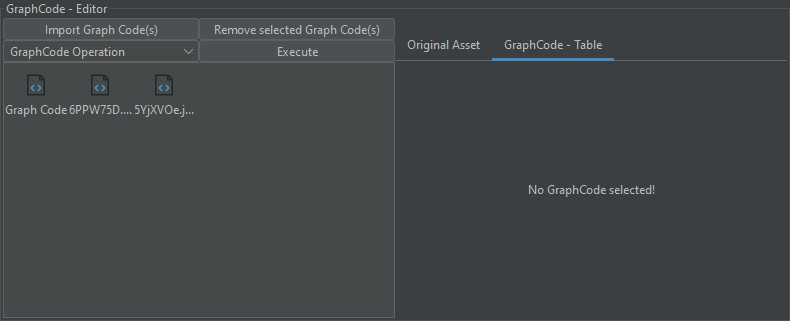
\includegraphics[width=\textwidth]{images/left_no_sel}
    \caption{Kein Graph Code ausgewählt.}
  \end{figure}

\end{frame}

\begin{frame}{Implementierung - Screenshots}

  \begin{figure}
    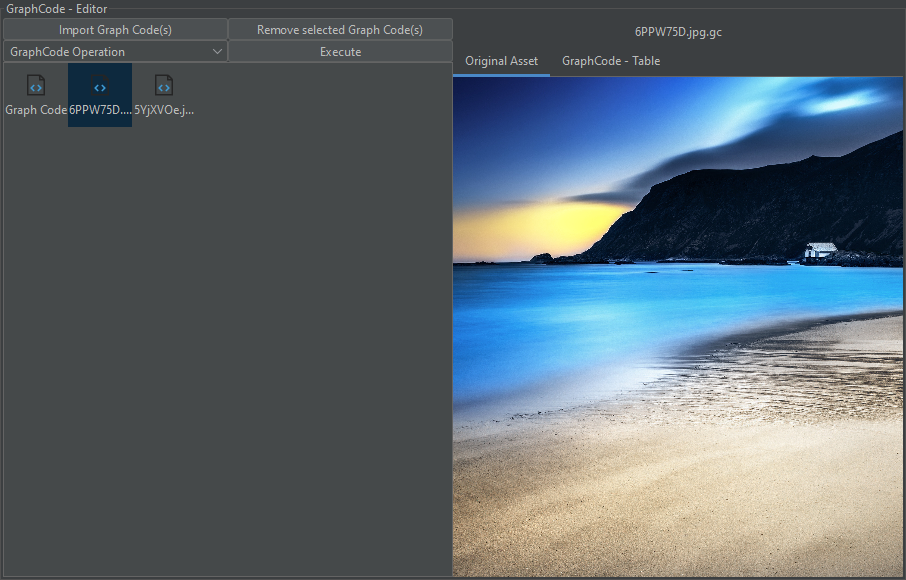
\includegraphics[width=0.9\textwidth]{images/left_sel_original}
    \caption{Graph Code ausgewählt, Darstellung der originalen Datei.}
  \end{figure}

\end{frame}

\begin{frame}{Implementierung - Screenshots}

  \begin{figure}
    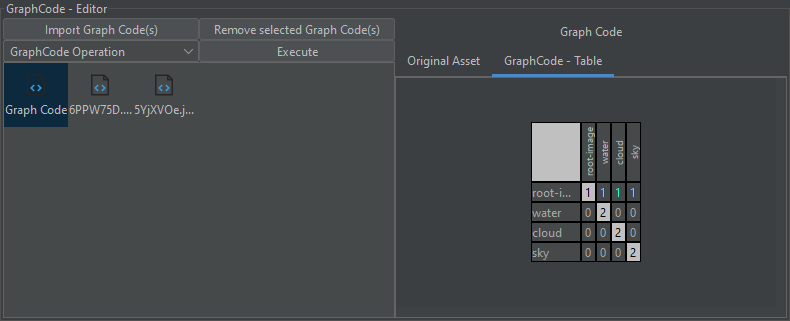
\includegraphics[width=\textwidth]{images/left_sel}
    \caption{Graph Code ausgewählt, tabellarische Darstellung des Graph Codes.}
  \end{figure}

\end{frame}

\begin{frame}{Implementierung - Screenshots}

  \begin{figure}
    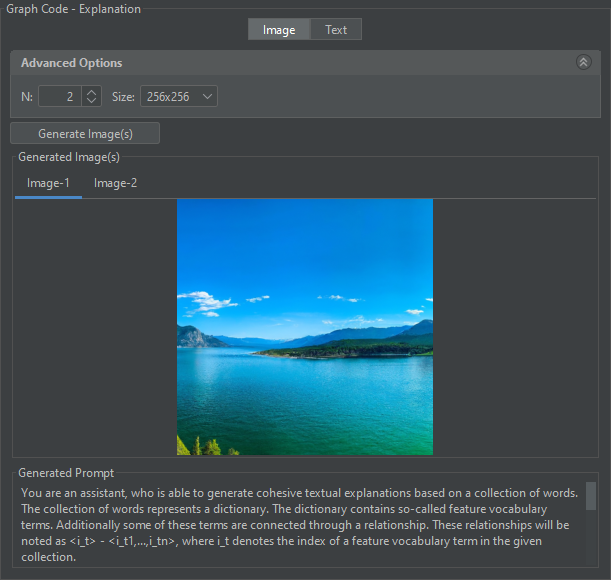
\includegraphics[width=0.6\textwidth]{images/right_img_two_exps_1}
    \caption{Erstes Bild zu ausgewähltem Graph Code generiert.}
  \end{figure}

\end{frame}

\begin{frame}{Implementierung - Screenshots}

  \begin{figure}
    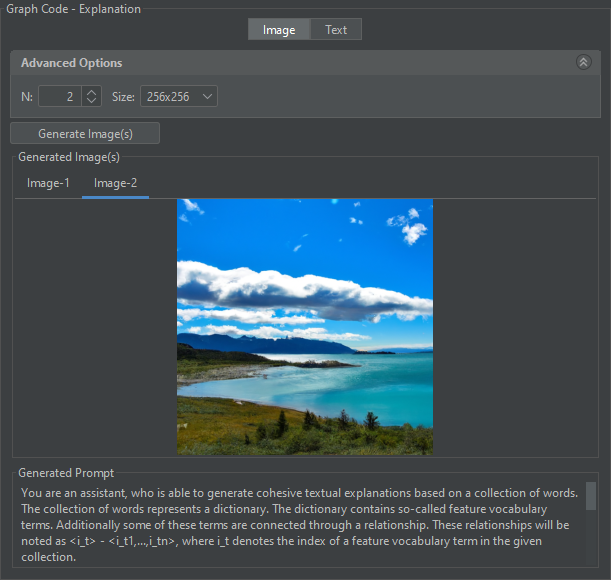
\includegraphics[width=0.6\textwidth]{images/right_img_two_exps_2}
    \caption{Zweites Bild zu ausgewähltem Graph Code generiert.}
  \end{figure}

\end{frame}

\begin{frame}{Implementierung - Screenshots}

  \begin{figure}
    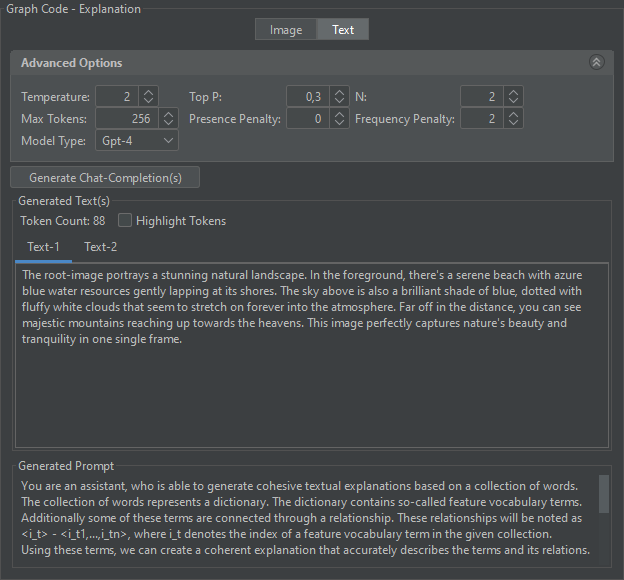
\includegraphics[width=0.6\textwidth]{images/right_text_two_exps_1}
    \caption{Erster Text zu ausgewähltem Graph Code generiert.}
  \end{figure}

\end{frame}

\begin{frame}{Implementierung - Screenshots}

  \begin{figure}
    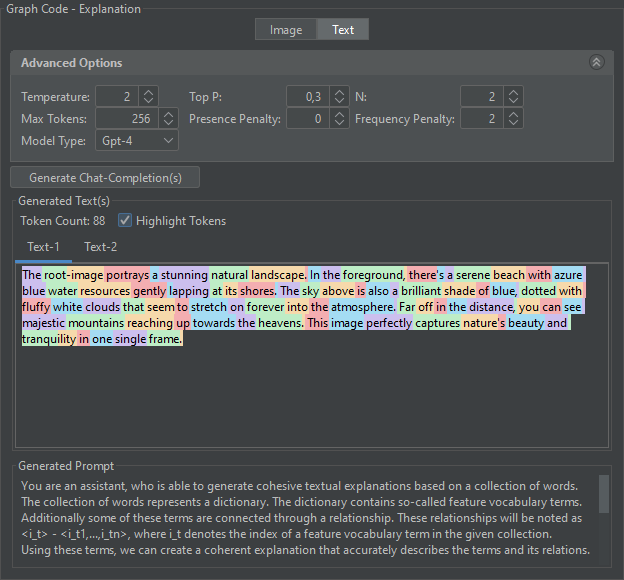
\includegraphics[width=0.6\textwidth]{images/right_text_two_exps_1_high}
    \caption{Hervorheben von Tokens beim ersten generierten Text.}
  \end{figure}

\end{frame}

\begin{frame}{Implementierung - Screenshots}

  \begin{figure}
    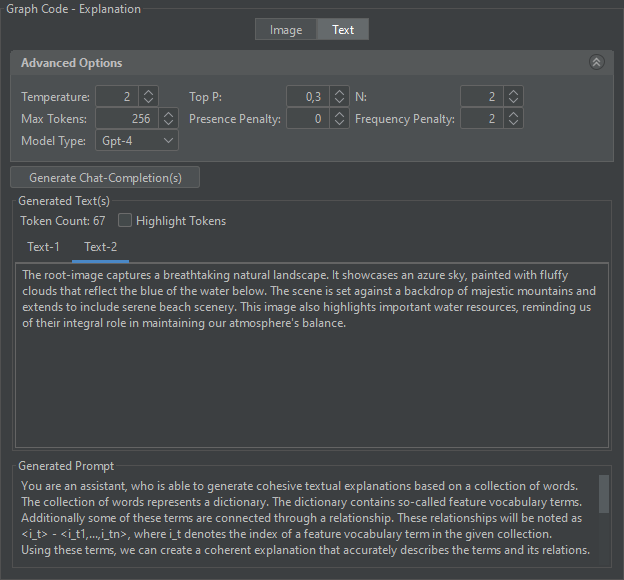
\includegraphics[width=0.6\textwidth]{images/right_text_two_exps_2}
    \caption{Zweiter Text zu ausgewähltem Graph Code generiert.}
  \end{figure}

\end{frame}

\section{Evaluierung}

\begin{frame}{Evaluierung}

  \begin{block}{FZ 1.4/E Erklärbarkeit von MMIR mittels gen. KI}
    \begin{itemize}
      \item Durchführung von \textbf{Exp. 1 - Interaktion mit GC's}
      \item Auswertung des Experiments
    \end{itemize}
  \end{block}

  \begin{exampleblock}{Erkenntnisse / Anpassungen}
    \begin{itemize}
      \item Kleinere Mängel entdeckt u. behoben
    \end{itemize}
  \end{exampleblock}

\end{frame}

\begin{frame}{Evaluierung}

  \begin{block}{FZ 2.4/E Integration generativer KI in das GMAF}
    \begin{itemize}
      \item Durchführung von \textbf{Exp. 2 - Erstellen einer Erklärung}
      \item Auswertung des Experiments
    \end{itemize}
  \end{block}

  \begin{exampleblock}{Erkenntnisse / Anpassungen}
    \begin{itemize}
      \item Layouts für Erklärungen angepasst
      \item Benutzungsschnittstelle für Erklärungen erweitert (n: Tabs)
      \item Visuelle Rückmeldung zum Status einer Anfrage
    \end{itemize}
  \end{exampleblock}

\end{frame}

\begin{frame}{Evaluierung}

  \begin{block}{Weitere Anpassungen}
    \begin{itemize}
      \item Gegenüberstellung der orig. Datei zum GC
      \item Hervorheben von Tokens
      \item Sichern von generierten Erklärungen in einem Ordner
      \item Neue Modelle GPT-4 u. Dall-E 3, sowie TTS (Text To Speech)
      \item Neue Benutzungsschnittstelle für TTS
    \end{itemize}
  \end{block}

\end{frame}

\begin{frame}{Evaluierung - Anpassungen}

  \begin{figure}
    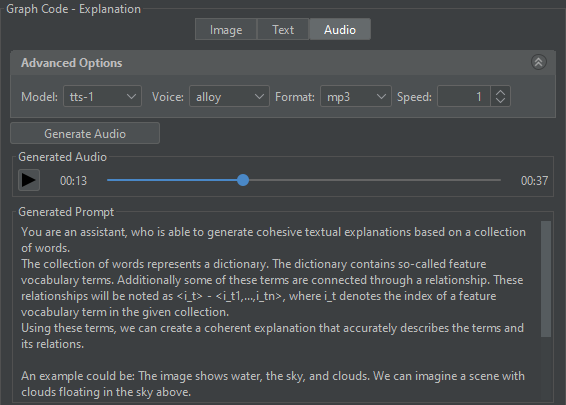
\includegraphics[width=0.75\textwidth]{images/right_audio_exp}
    \caption{Neue Benutzungsschnittstelle für TTS zum Generieren von auditiven Erklärungen.}
  \end{figure}

\end{frame}

\section{Zusammenfassung}

\begin{frame}{Zusammenfassung}

  \begin{block}{Eine Herausforderung ist...}
    \begin{itemize}
      \item Gen. KI (komplexere) Aufgaben mittels Instruktionen zu vermitteln
    \end{itemize}
    %Generativer KI Aufgaben mittels Instruktionen zu vermitteln (Zufälligkeitsfaktor, jede generierte Antwort kann im Wortlaut individuell sein).
  \end{block}

  \begin{block}{Stolpersteine}
    Keine Stolpersteine während der Bearbeitung der Arbeit erfahren
  \end{block}

\end{frame}

\begin{frame}{Zusammenfassung}

  \begin{exampleblock}{Arbeitsergebnisse / ziele}
    \begin{itemize}
      \item Anwendung löst bestehende Verfahren durch gen KI ab
      \item Anwendung ermöglicht durch Integration gen KI andere Ausgabemodalitäten
      \item Anwendung ermöglicht das Generieren ähnlicher MMIR Inhalte
    \end{itemize}
  \end{exampleblock}

\end{frame}

\end{document}
